\chapter{Clustering Hard et Soft}
\minitoc
\thispagestyle{empty}
\newpage

\section{Introduction}
Le clustering est un moyen de classer les données brutes de manière raisonnable et de rechercher les modèles cachés qui peuvent exister dans les ensembles de données \cite{huang1998extensions}.
Le clustering est une méthode de l’apprentissage automatique non-supervisé et un outil mathématique qui tente de découvrir des structures ou certains modèles dans un jeu de données, où les objets à l'intérieur de chaque cluster montrent un certain degré de similitude \cite{sasirekha2013agglomerative}. Le but de l'analyse de cluster consiste à partitionner un ensemble de \(\displaystyle N \) objets en clusters de sorte que les objets dans le cluster doivent être similaires les uns aux autres et les objets dans différents groupes doivent être différents avec les uns des autres \cite{yang1993survey}. Il peut être réalisé par divers algorithmes qui diffèrent considérablement dans leur notion de ce qui constitue un cluster et comment les trouvés efficacement. L'analyse de cluster est un processus itératif de découverte de connaissances ou d'optimisation multi-objectifs interactive \cite{sasirekha2013agglomerative}. Les chercheurs ont mis au point de nombreux algorithmes de clustering, qui ont été largement appliqués. Ils peuvent être globalement classés en deux groupes : partitionnelle et hiérarchique. Les algorithmes de partition traitent les données d'entrée et créent une partition qui regroupe les données en clusters. En revanche, les algorithmes hiérarchiques créent un ensemble de partitions imbriquées appelé hiérarchie de cluster \cite{zhou2016method}. En général, un algorithme de clustering hiérarchique partitionne un ensemble de données en différents clusters via une agglomération ou une approche divisive basée sur un dendrogramme \cite{zhong2011minimum}.
Les concepts du clustering incluent des groupes avec de petites distances entre les membres du cluster, des zones denses, des intervalles ou des distributions statiques particulières.

Le clustering est donc une méthode qui cherche à minimiser l’inertie intra-cluster et maximiser l’inertie inter-cluster.Pour minimiser l’inertie intra-cluster et maximiser l’inertie inter-cluster, les algorithmes de clustering utilise des métriques pour mesurer la distance entre les clusters et les critères de liaison qui sont la façon dont la distance entre les clusters est calculée. \\

Avant de rentrer directement sur le fonctionnement des algorithmes de clustering, nous verrons d’abord les métriques et les critères de liaison qui sont utiliser dans le processus du clustering ensuite le clustering hiérarchique, partitionnel et l’indice de validité du clustering.
\section{Les métriques}
Le choix d'une métrique appropriée influencera la forme des grappes, car certains éléments peuvent être relativement plus proches les uns des autres sous une métrique que dans une autre.
Par exemple, en deux dimensions, sous la métrique de distance Manhattan, la distance entre l'origine (0,0) et (.5, .5) est la même que la distance entre l'origine et (0, 1), tandis que sous le distance euclidienne métrique, cette dernière est strictement supérieure. \\
Certaines métriques couramment utilisées pour le clustering hiérarchique sont :

\begin{table}[!htbp]
    \centering
	\begin{tabular}{|c| c|}
	\hline
	\rowcolor{blueforest}
	\color{white} \textbf{Names} & \color{white} \textbf{Formula}  \\ \hline
	Euclidean  & \(\displaystyle \left\lVert a - b\right\rVert_{2} = \sqrt{\sum_{i}^{} (a_{i} - b_{i})^{2} } \)   \\  \hline
	Squared Euclidean distance  & \(\displaystyle \left\lVert a - b\right\rVert_{2}^{2} = \sum_{i}^{} (a_{i} - b_{i})^{2} \)   \\  \hline
	Manhattan distance  & \(\displaystyle \left\lVert a - b\right\rVert_{1} = \sum_{i}^{} \left\lvert a_{i} - b_{i} \right\rvert \)   \\  \hline
	Maximum distance  & \(\displaystyle \left\lVert a - b\right\rVert_{\infty} = \max_{i} \left\lvert a_{i} - b_{i} \right\rvert  \)   \\  \hline
	Mahalanobis distance  & \(\displaystyle \sqrt{(a-b)^{T}S^{-1}(a-b)} \) where S is the Covariance matrix   \\  \hline
	\end{tabular}
	\caption{Les métriques }
	\label{metrics}
\end{table}

\section{Critère de liaison}
Le critère de liaison détermine la distance entre les ensembles d'observations en fonction des distances par paires entre observations. Certains critères de liaison couramment utilisés entre deux ensembles d’observations A et B sont : \ref{linkage_criteria}

\begin{table}[!htbp]
    \centering
	\begin{tabular}{|c| c|}
	\hline
	\rowcolor{blueforest}
	\color{white} \textbf{Names} & \color{white} \textbf{Formula}  \\ \hline
	\makecell{Maximum or \\ complete-linkage clustering}   & \(\displaystyle \max \{d(a,b): a \in A,b \in B \} \)   \\  \hline
	\makecell{Minimum or \\ single-linkage clustering}   & \(\displaystyle \min \{d(a,b): a \in A,b \in B \} \)   \\  \hline
	\makecell{ Unweighted average linkage \\ clustering (or \textbf{UPGMA})} & \(\displaystyle \frac{1}{ \left\lvert A\right\rvert  \cdot \left\lvert B\right\rvert } \sum_{a \in A} \sum_{b \in B} d(a,b)  \)   \\  \hline
	\makecell{Weighted average linkage \\ clustering (or \textbf{WPGMA})}  & \(\displaystyle d(i \cup j,k) = \frac{d(i,k)+d(j,k)}{2} \)   \\  \hline
	\makecell{Centroid linkage clustering,\\ or \textbf{UPGMC}}   & \makecell{\(\displaystyle \left\lVert c_{s} - c_{t} \right\rVert \) where \(\displaystyle c_{s} \) and \(\displaystyle c_{t} \)  are the \\ centroids of clusters  \(\displaystyle s \) and \(\displaystyle t \), respectively.}   \\  \hline
	Minimum energy clustering  & \(\displaystyle \frac{2}{nm}\sum_{i,j=1}^{n,m} \left\lVert
	a_{i} - b_{j}\right\rVert^{2} - \frac{1}{n^{2}} \sum_{i,j=1}^{n} \left\lVert
	a_{i} - a_{j}\right\rVert^{2}  - \frac{1}{m^{2}} \sum_{i,j=1}^{m} \left\lVert
	b_{i} - b_{j}\right\rVert^{2}   \)   \\  \hline
	\end{tabular}
	\caption{Les critères de liaison }
	\label{linkage_criteria}
\end{table}

Puisque le clustering est une méthode qui cherche à minimiser l'inertie au sein des clusters et à maximiser l'inertie entre les clusters, il existe donc deux types de distance, celle entre les objets des différents clusters qui est la distance inter-cluster et celle entre les objets du même cluster qui est la distance intra-cluster. Comme le montre la figure \ref{inter_intra_clusters}.

\begin{figure}[H]
	\begin{center}
		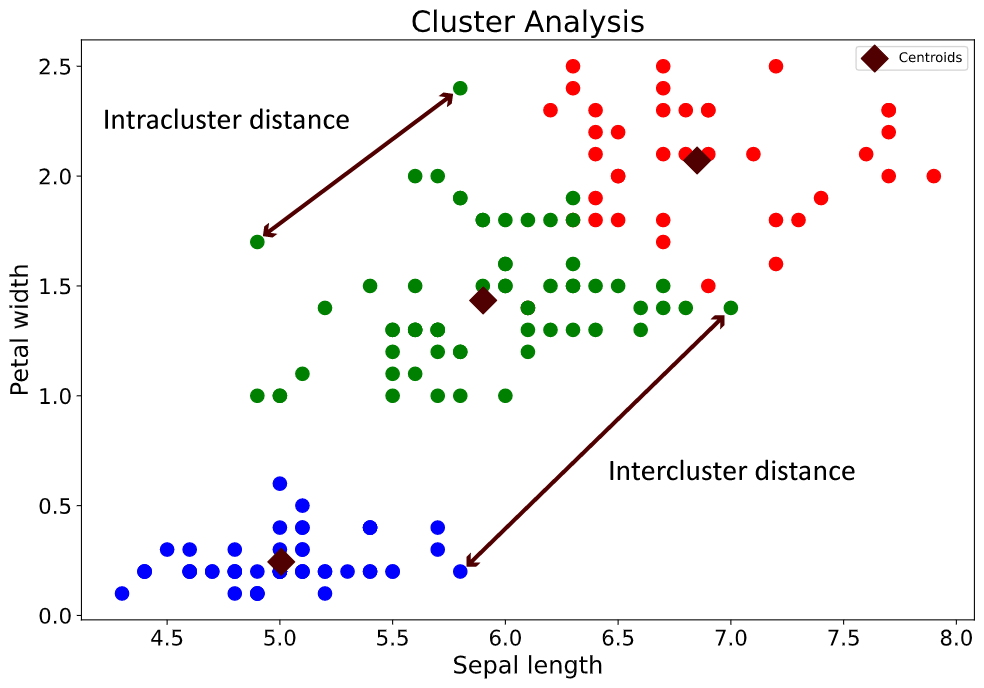
\includegraphics[scale=0.3]{images/chapitre6/iris_inter_intra_clusters.png}
	\end{center}
\caption{Distances intracluster et intercluster.}
\label{inter_intra_clusters}
\end{figure}

\subsection{Distance inter-cluster}
La distance inter-cluster est la distance entre deux objets appartenant à deux clusters différents. Il y’a 5 types de distance inter-cluster :

\subsubsection{Distance de liaison unique}
La distance de liaison unique est la distance la plus proche entre deux objets appartenant à deux clusters différents. Le clustering de liaison unique est basé sur le critère de connectivité. La distances entre deux clusters \(\displaystyle S \) et \(\displaystyle T \) est : \cite{maulik2002performance}

% \begin{figure}[!h]
%     \centering
%     \subfloat[\centering les points de données en 2 dimensions]{{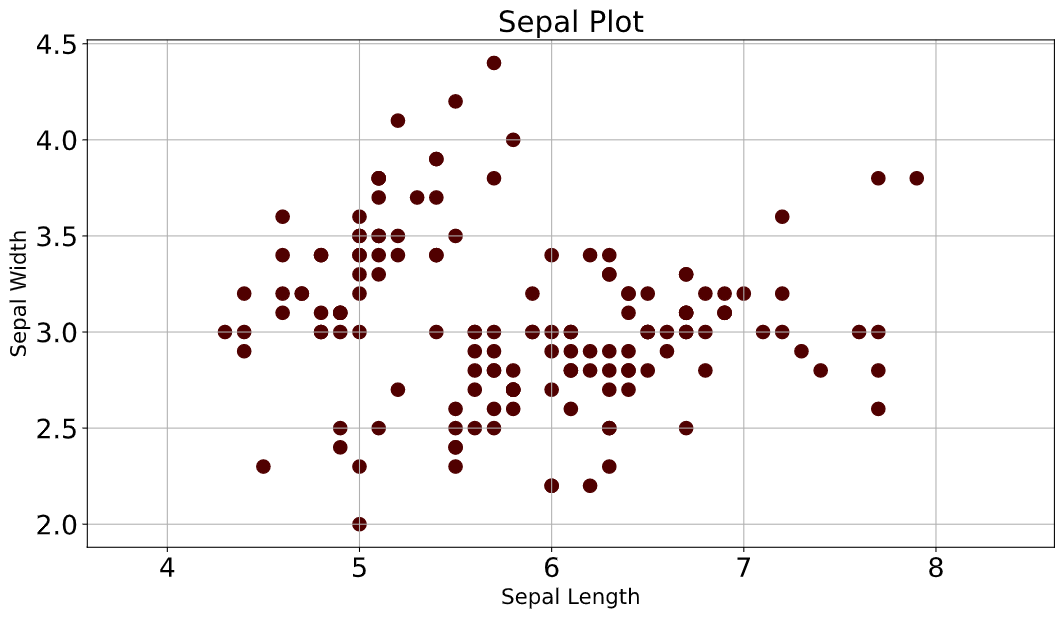
\includegraphics[width=7cm]{images/chapitre6/data_for_fuzzy.png} \label{data_for_fuzzy} }}%
%     \qquad
%     \subfloat[\centering Dendrogramme]{{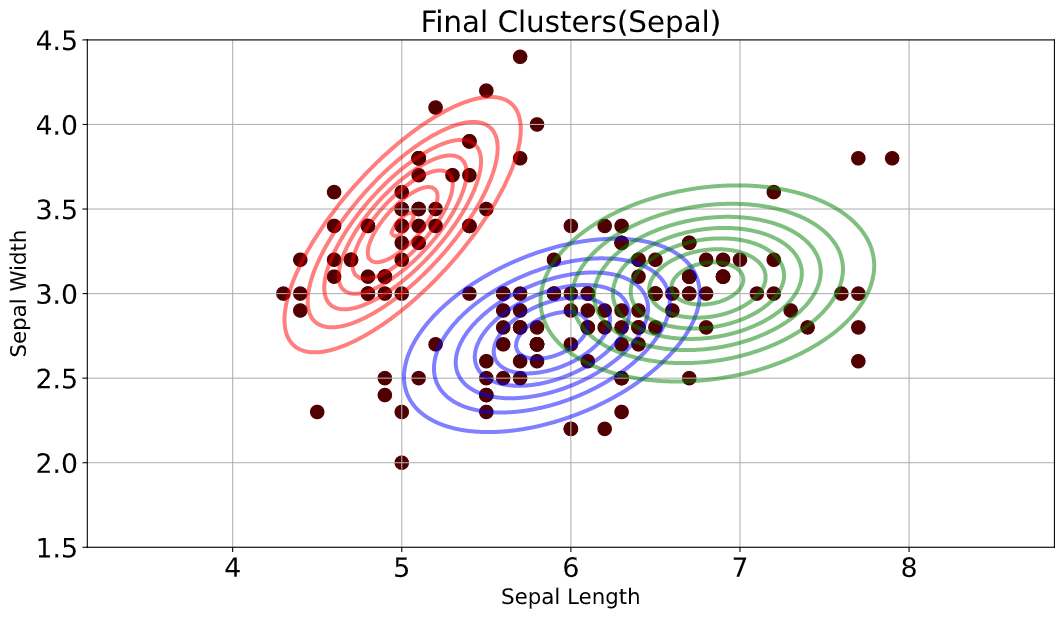
\includegraphics[width=7cm]{images/chapitre6/fuzzyExemple.png} } \label{fuzzy_example}}%
%     %\caption{Dendrogramme}%
% \end{figure}

\begin{equation}
	\vcenter{\hbox{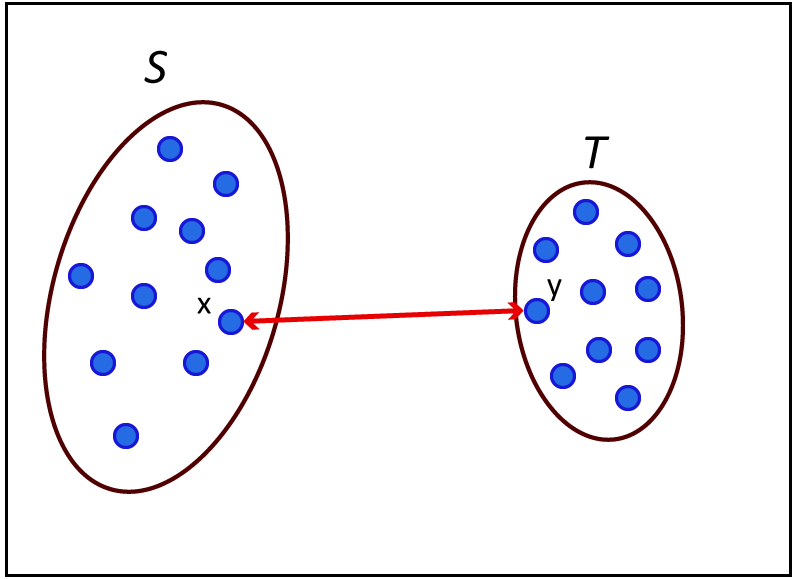
\includegraphics[scale=0.2]{images/chapitre6/single_linkage.png}}}
	\qquad
	\begin{aligned}
		 \delta (S,T) = \min  \Bigg\{
	\begin{tabular}{@{}l@{}}
		\(\displaystyle d(x,y) \)  \\
		\(\displaystyle x \in S,y \in T \) 
	\end{tabular} \Bigg\}
	\end{aligned}
	\label{signle_linkage_illust}
\end{equation}
% \begin{figure}[H]
% 	\begin{center}
% 		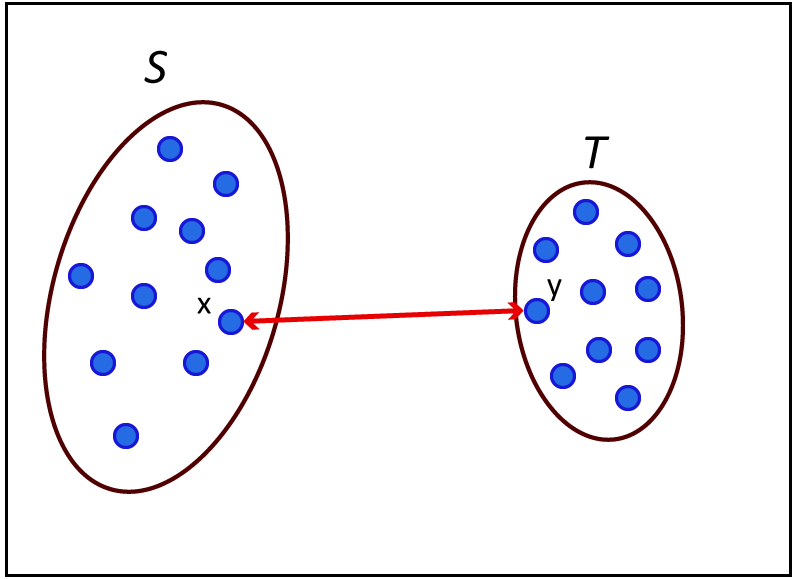
\includegraphics[width=\textwidth]{images/chapitre6/single_linkage.png}
% 	\end{center}
% \caption{Distances intracluster et intercluster.}
% \label{signle_linkage_illust}
% \end{figure}

% \begin{equation}
%      \delta (S,T) = \min  \Bigg\{
% \begin{tabular}{@{}l@{}}
%     \(\displaystyle d(x,y) \)  \\
%     \(\displaystyle x \in S,y \in T \) 
% \end{tabular} \Bigg\}
% \end{equation}

Le principal avantage de la liaison simple est qu'elle peut gérer des formes non elliptiques \cite{kumar2014performance}. Cependant, il est sensible au bruit et aux valeurs aberrantes \cite{jain1988algorithms} \cite{pang2005introduction}.

\subsubsection{Distance de liaison complète}
La distance de liaison complète est la distance entre deux objets les plus éloignés appartenant à deux clusters différents. La liaison complète est la plus grande distance entre les points de données dans deux clusters S et T définit par la formule suivante :

\begin{equation}
	\vcenter{\hbox{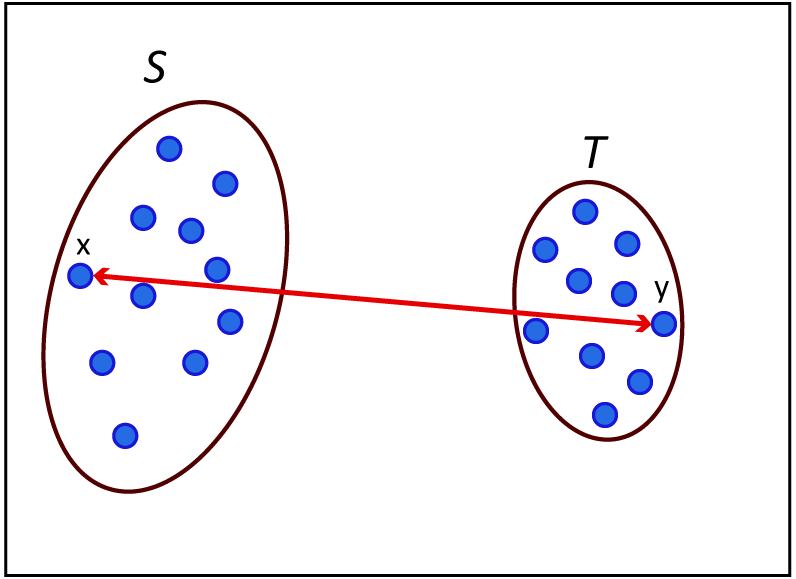
\includegraphics[scale=0.2]{images/chapitre6/complet_linkage.png}}}
	\qquad
	\begin{aligned}
		\delta (S,T) = \max  \Bigg\{
	\begin{tabular}{@{}l@{}}
	\(\displaystyle d(x,y) \)  \\
	\(\displaystyle x \in S,y \in T \) 
	\end{tabular} \Bigg\}
	\end{aligned}
	\label{complet_linkage_illust}
\end{equation}


% \begin{figure}[H]
% 	\begin{center}
% 		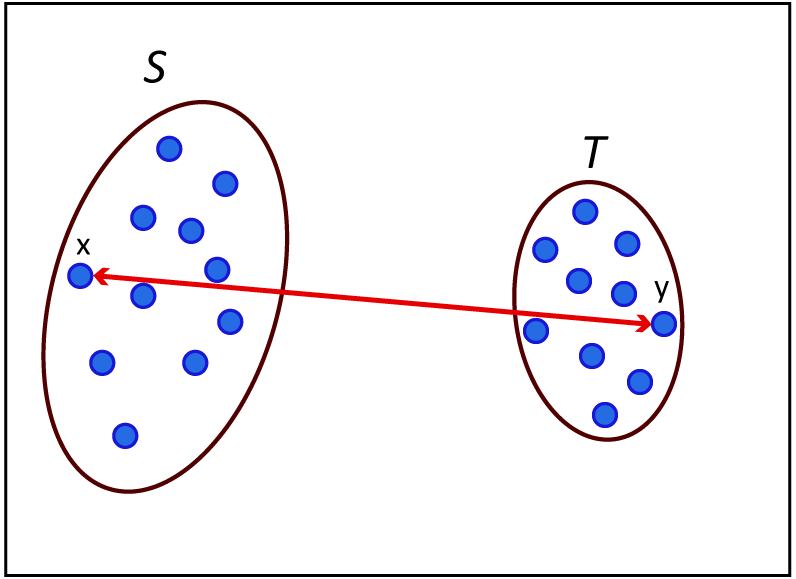
\includegraphics[width=\textwidth]{images/chapitre6/complet_linkage.png}
% 	\end{center}
% \caption{Distances intracluster et intercluster.}
% \label{complet_linkage_illust}
% \end{figure}

% \begin{equation}
% 	\delta (S,T) = \max  \Bigg\{
% \begin{tabular}{@{}l@{}}
%    \(\displaystyle d(x,y) \)  \\
%    \(\displaystyle x \in S,y \in T \) 
% \end{tabular} \Bigg\}
% \end{equation}

Cette distance ne tient pas compte de la structure du cluster et ne peut pas détecter les amas non sphériques \cite{kumar2014performance}.
\subsubsection{Distance de liaison moyenne}
La distance de liaison moyenne est la distance moyenne entre tous les objets appartenant à deux clusters différents. Le clustering de liaison moyenne a une procédure similaire que celle à liaison unique sauf le calcul de la distance entre deux clusters. Il utilise la moyenne entre les points de deux clusters S et T comme suit \cite{kumar2014performance} :

\begin{equation}
	\begin{split}
		\delta (S,T) = \frac{1}{\left\lvert S \right\rvert \left\lvert T \right\rvert  } \sum_{_{ x \in S},_{y \in T}} d(x,y)  \\
	\end{split}
\end{equation}
Le clustering utilisant la liaison moyenne est moins sensible au bruit et aux valeurs aberrantes. Le seul inconvénient est sa polarisation vers les amas globulaires \cite{pang2005introduction}.

\subsubsection{Centroïde Linkage Distance}
La distance de liaison centroïde est la distance entre les centres vs et vt de deux clusters S et T respectivement, définie comme :

\begin{equation}
	\begin{tabular}{@{}l@{}}
		\(\displaystyle \delta (S,T) = d(v_{s}, v_{t} ) \) où \\ \\
		\(\displaystyle v_{s} = \frac{1}{\left\lvert S \right\rvert}  \sum_{x \in S} x,v_{t} = \frac{1}{\left\lvert T \right\rvert} \sum_{y \in T}y  \) 
	\end{tabular} 
\end{equation}

\subsubsection{Distance de liaison moyenne du centre de gravité}
La distance de liaison moyenne du centre de gravité est la distance entre le centre d'un cluster et tous les objets appartenant à un autre cluster, définie comme :

\begin{equation}
	\delta (S,T) = \frac{1}{\left\lvert S \right\rvert  + \left\lvert T \right\rvert  }  \Bigg\{
\begin{tabular}{@{}l@{}}
   \(\displaystyle \sum_{x \in S} d(x,vt) + \sum_{y \in T}d(y,vs) \)
\end{tabular} \Bigg\}
\end{equation}

\subsection{Distance intra-cluster}
La distance intra-cluster est la distance entre deux objets appartenant au même cluster. Il y’en a trois types :

\subsubsection{Distance de diamètre complet}
La distance de diamètre complet est la distance entre deux objets les plus éloignés appartenant au même cluster défini comme :

\begin{equation}
	\begin{split}
		\Delta (S) = \max_{x,y \in S} \{ d(x,y) \}  \\
	\end{split}
\end{equation}

\subsubsection{Distance de diamètre moyen}
La distance de diamètre moyen est la distance moyenne entre tous les objets appartenant au même cluster défini comme :

\begin{equation}
	\begin{split}
		\Delta (S) = \frac{1}{\left\lvert S \right\rvert \cdot  (\left\lvert S \right\rvert - 1)} \sum_{x,y \in S ; x \neq y} \{ d(x,y) \} \\
	\end{split}
\end{equation}

\subsubsection{Diamètre barycentre Distance}
La distance de diamètre barycentre est à double distance moyenne entre tous les objets et le centre de groupe de s défini comme :

\begin{equation}
	\Delta (S) = 2  \Bigg \{
	\frac{\sum_{x \in S}d(x,\overline{v})}{\left\lvert S \right\rvert } \Bigg\} 
	\hspace{20pt} où \hspace{10pt} \overline{v} = \frac{1}{\left\lvert S \right\rvert} \sum_{x \in S}x
\end{equation}

\section{Le clustering hiérarchique}
\subsection{Introduction}
Dès les années 1970, on a estimé qu'environ 75\% de tous les travaux publiés sur le clustering utilisaient des algorithmes hiérarchiques \cite{murtagh2012algorithms}. Le clustering hiérarchique est une méthode de clustering qui permet d’identifier des clusters dans un ensemble de données. Contrairement aux autres méthodes de clustering comme le k-means, le clustering hiérarchique n’oblige pas à spécifier à l’avance le nombre de clusters à générer. Et le résultat est une représentation arborescente des observations, appelée dendrogramme. L'interprétation des informations contenues dans un dendrogramme est souvent d'un ou plusieurs types : relations d'inclusion d'ensemble, partition des ensembles d'objets et clusters significatifs \cite{murtagh2012algorithms}. C’est une méthode de clustering d’apprentissage automatique non supervisé qui procède à une décomposition de données en cherchant à construire une hiérarchie de clusters. Cette méthode suit deux approches basées sur la direction du progrès, c'est-à-dire s'il s'agit du flux descendant ou ascendant de création de clusters. Il s'agit respectivement de l'Approche Divisive et de l'Approche Agglomérative. \\
Le clustering agglomératif commence à partir des clusters singleton et obtient une hiérarchie en fusionnant successivement les clusters, tandis que le clustering divisif commence par un cluster unique contenant tous les points et se poursuit en fractionnant les clusters de manière itérative \cite{gurrutxaga2010sep}. le clustering hiérarchique crée donc une décomposition hiérarchique de l'ensemble de données.

\subsection{Clustering hiérarchique agglomératif}
En clustering, l'un des algorithmes les plus largement utilisés est les algorithmes agglomératifs. Il s'agit d'une approche « ascendante » : chaque observation commence dans son propre cluster, et les paires de clusters sont fusionnées au fur et à mesure que l'on monte dans la hiérarchie. Les résultats de la classification hiérarchique sont généralement présentés dans un dendrogramme. Cependant, pour certains cas particuliers, des méthodes agglomératives efficaces optimales (de complexité) sont connues : SLINK pour une liaison simple et CLINK pour un clustering à liaison complète \cite{sasirekha2013agglomerative}.
L’algorithme de clustering AHC a trois mesures de distance principales : liaison unique, liaison complète et liaison moyenne. Il est également appelé l’algorithme de clustering du plus proche voisin lorsque le critère single-linkage (liaison unique) est utilisée pour mesurer la distance distance entre les clusters \cite{zhou2016method}.
Dans le clustering hiérarchique agglomératif classique, une paire de clusters à fusionner à la distance minimale inter-cluster \cite{wu2004clustering}.

\subsubsection{Exemple de clustering agglomératif}

Par exemple, supposons que les données de la figure \ref{agglo_clustering} doivent être regroupées et que la métrique de distance est la distance euclidienne.
Le dendrogramme obtenu après le clustering serait comme la celui de la figure \ref{dendrogramme} \\
Et pour obtenir le nombre de clusters optimal avec le dendrogramme, la méthode la plus connue est celle qui cherche la distance verticale la plus élevée qui ne croise aucun cluster et les lignes verticales franchissent le seuil représente le nombre optimal de clusters. En utilisant le dendrogramme précédant on obtient 2 clusters comme le montre la figure \ref{dendrogramme}.

\begin{figure}[H]
	\centering
    \subfloat[\centering Les éléments du dataset.]{{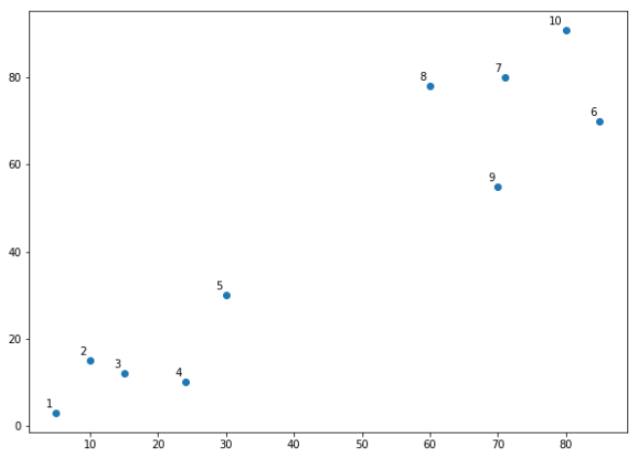
\includegraphics[width=7cm]{images/chapitre6/agglo_clustering.png} \label{agglo_clustering} }}%
    \qquad
    \subfloat[\centering Le dendrogramme.]{{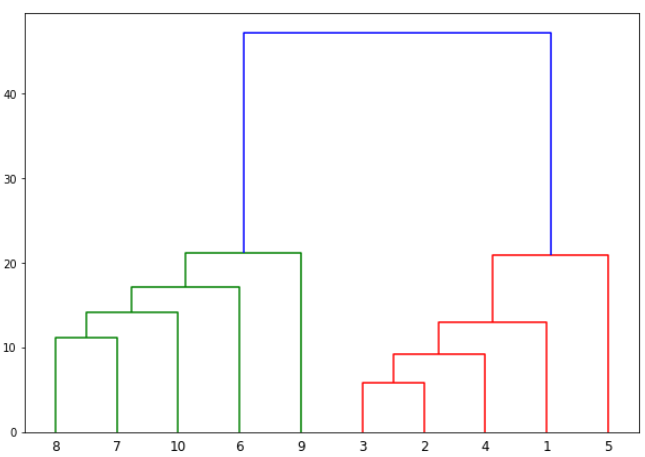
\includegraphics[width=7cm]{images/chapitre6/dendrogram.png} } \label{dendrogramme}}%
    %\caption{Dendrogramme}%
\end{figure}


\subsection{Clustering hiérarchique divisive}
Le principe de base du clustering divisif a été publié sous le nom d'algorithme DIANA (Divisive Analysis Clustering) \cite{Finding_Groups_in_Data_An_Introduction_To_Cluster_Analysis}. Contrairement au clustering hiérarchique agglomératif, le clustering hiérarchique divisif suit une approche descendante dans laquelle tous les points de données appartiennent à un seul grand cluster et celui-ci est divisé en groupes plus petits en fonction d'une logique de terminaison ou d'un point au-delà duquel il n'y aura plus de division de points de données. Le principe du clustering divisif est illustrer par la figure ci-dessous. \\
Le fractionnement est effectué de manière récursive au fur et à mesure que l'on descend dans la hiérarchie et il existe \(\displaystyle 2^{n-1}-1 \) \cite{edwards1965method}  façons de diviser un ensemble de n objets en deux sous-ensembles \cite{roux2018comparative}. Par conséquent le fractionnement prend top du temps sur la recherche de toutes les bipartitions possibles. Le clustering hiérarchique divisif procède par le fractionnement des clusters en deux clusters les moins similaires en utilisant des critères de type distance ou rapport et ensuite détermine les niveaux des nœuds (qui représente les groupes obtenus dans le dendrogramme).

\begin{figure}[H]
	\begin{center}
		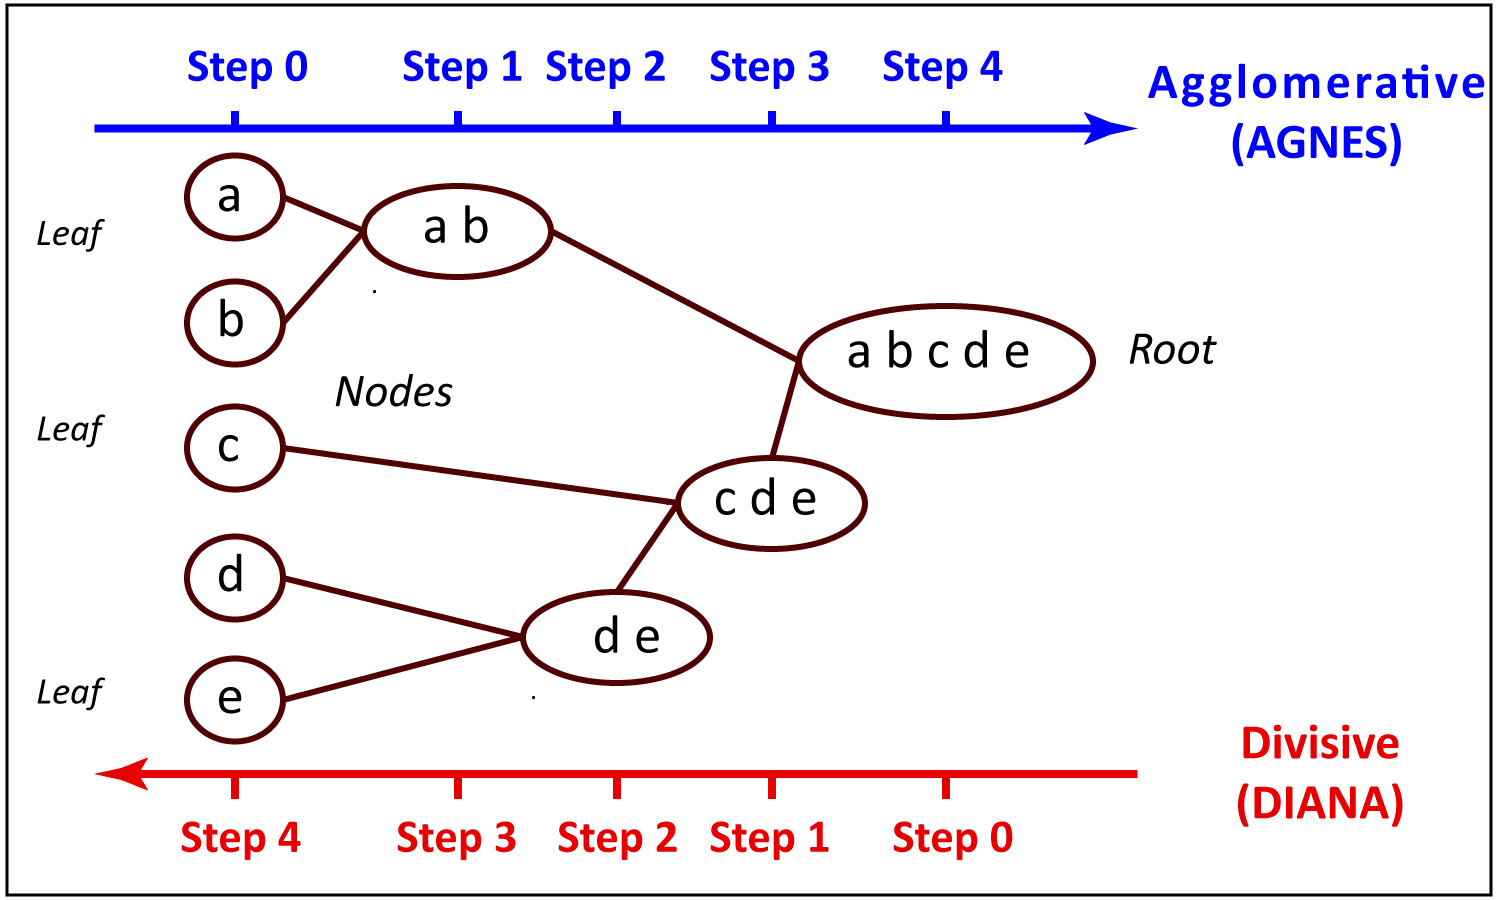
\includegraphics[scale=0.15]{images/chapitre6/hierarchical_agglo_divisive.png}
	\end{center}
\caption{La direction du clustering hiérarchique agglomérative et divisive.}
\label{hierarchical_agglo_divisive_illust}
\end{figure}

\subsection{Procédures de fractionnement des clusters}
Un certain nombre de procédures de fractionnement ont été conçus dans le passé. La procédure de Williams Et Lambert (1959) \cite{williams1959multivariate} est dite monothéique dans le sens où les ensembles d’objets sont divisé en fonction des valeurs d’une seule variable. Cette idée a été mise à jour en utilisant une composante principale au lieu d’une seule variable (algorithme Principal Directions Divisive Partitioning ou PDDP par Boley 1997) \cite{roux2018comparative}. \\
Une autre approche pour contourner la complexité du fractionnement consiste à extraire un ou plusieurs objets, de l’ensemble à fractionner. Macnaughton-Smith et al. (1964) \cite{macnaughton1964dissimilarity} ont proposé de sélectionner l’objet le plus distant comme center d’un nouveau cluster éloigné, puis les objets (les éléments du data set) les plus proche s’agrègent vers ce nouveau cluster \cite{roux2018comparative}. \\
Une idée similaire a été développée par Hubert (1973) \cite{hubert1973monotone}, qui suggéré d’utiliser une paire d’objets comme point d’origine de la nouvelle bipartition. Son choix a été de sélectionner les deux objets qui sont les plus dissemblables, puis de construire les deux sous-clusters en fonction des distances à ces points d’origines \cite{roux2018comparative}. \\
Exploitant cette idée, Roux \cite{roux1991basic} \cite{roux1995divisive} considérait les bipartitions générées par toutes les paires d'objets, en conservant la bipartition avec la meilleure évaluation de certains critères a priori \cite{roux2018comparative}. \\

\subsection{Evaluations des bipartitions}
Quel que soit le critère retenu, une série de très bonnes bipartitions ne se traduit pas automatiquement par une bonne hiérarchie. Les critères qui permettent d’évaluer les bipartitions sont de deux types : critère de type distance et les critères de type rapport. L’idée est donc de prendre en compte non seulement les dissemblances entre les clusters, mais aussi les dissemblances avec les éléments de deux clusters. Ces critères qui sont appelé aussi indice de validité sont énoncé dans le tableau \ref{validity_index_hard}.

\subsection{Déterminations de niveaux de nœuds }
Pour l’algorithme agglomératif, la valeur de l’indice de validité obtenu pour l’estimation du nombre optimale de clusters devient le niveau du nœud correspondant, et le dendrogramme ne montre aucun croisement (ou inversion) des branches. Malheureusement, les procédures qui divisent, en général, ne bénéficient pas de cette propriété, en raison du non-optimalité des fractionnements successifs. Une règle est alors nécessaire pour obtenir des niveaux cohérents et une véritable représentation arborescente \cite{roux2018comparative}.
\subsection{Conclusion}
Le clustering hiérarchique dans la recherche d'informations identifie donc des groupements ou regroupements des « objets » étudiés qui représentent le mieux certaines relations de similitude. Il permet ainsi d’obtenir des résultats dans une hiérarchie de cluster appelé dendrogramme. Et si le dendrogramme ne présente aucun croisement des branches, la visualisation de ce dernier permet de voir comment les différents sous-clusters sont liés les uns aux autres et à quelle distance sont les points de données.
\section{Le clustering partitionnel}

\subsection{K-means clustering}
K-means est un algorithme de clustering qui est largement utiliser pour analyser les clusters des grands ensembles de données. Il a été proposé par MacQueen en 1967 et c’était l’un des algorithmes d’apprentissage non supervisé le plus simple, qui a été appliqué pour résoudre les problèmes du clustering \cite{sun2008clustering}. Il s'agit d'un algorithme de partitionnement des clusters qui consiste à classer les objets d’un jeu de donnés en k clusters différents, de telle sorte que les clusters générés sont compacts et indépendants \cite{na2010research}.

\subsubsection{Le fonctionnement de l’algorithme k-means}
K-Means clustering fonctionne de cette façon : par exemple pour regrouper les données en trois clusters on commence par placer trois point appelé centroïde au hasard dans le jeu de données ensuite on affecte chaque point de data set au centroïde le plus proche ce qui nous donne trois clusters puis on déplace chaque centroïde au milieu de son cluster, on recommence jusqu’à ce que les centroïdes converge vers une position d’équilibre. L’algorithme requière donc à l’initialisation le nombre k de cluster à générer et k centroïdes (les centre des clusters) sont initialise avec des coordonnées aléatoires.

\subsubsection{Les étapes de l’algorithme}
L’algorithme de K-means clustering est un algorithme itératif qui procède comme suit :

\begin{itemize}
	\item	Sélection de k clusters a génère, où la valeur k est fixée à l'avance.
	\item	Initialisation des centroïdes avec de coordonnées aléatoires.
	\item	Calcul de la distance entre les objets et le centre de gravité du cluster.
	\item	Affectation des points au centroïde le plus proche.
	\item	Déplacement du centroïde à la moyenne du cluster.
	\item	Répétition des étapes précédente jusqu'à ce qu'il n'y ait pas de changement au centre des clusters.
\end{itemize}

Les étapes sont illustrées par la figure ci-dessous.

\begin{figure}[H]
	\begin{center}
		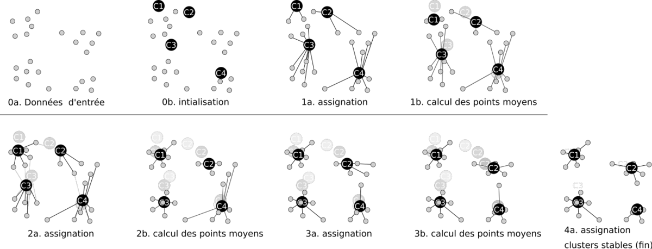
\includegraphics[width=\textwidth]{images/chapitre6/kmeans_steps.png}
	\end{center}
	\caption{Les étapes de l'algorithme k-means.}
	\label{kmeans_steps}
\end{figure}

Apres l’initialisation du nombre k des clusters a trouvées dans le jeu de données et k centroïdes, la distance euclidienne est généralement considérée pour déterminer la distance entre chaque objet de données et les centres du cluster. Cette distance est utilisée pour regrouper chaque objet de données au centre le plus proche \cite{fahim2006efficient}. La distance euclidienne entre un vecteur \(\displaystyle X = (x_{1},x_{2},x_{3},.....,x_{n}) \)  et un autre vecteur \(\displaystyle Y = (y_{1},y_{2},y_{3},.....,y_{n}) \), La distance euclidienne \(\displaystyle d(x_{i},y_{i})\) peut être obtenue comme suit:
\begin{equation}
    d(x_{i}, y_{i}) = \left[\sum_{i=1}^{n}(x_{i} - y_{i})^{2} \right]^{\frac{1}{2}}
\end{equation}

Lorsque tous les objets de données sont inclus dans certains clusters, la première étape est terminée et un regroupement précoce est effectué. Ce processus itératif continue jusqu'à ce que la fonction de critère est minimisé. \cite{na2010research}. \\
En supposant que l'objet cible est \(\displaystyle x \),\(\displaystyle x_{i} \) indique la moyenne du cluster \(\displaystyle C_{i} \), la fonction critère est définie comme suit :

\begin{equation}
    E = \sum_{i=1}^{k} \sum_{x \in C_{i}} \left\lvert x - x_{i} \right\rvert^{2}
\end{equation}

\subsubsection{Les lacunes de l’algorithme k-means}
L'algorithme de clustering k-means converge toujours vers le minimum local. Avant qu’il ne converge, l'algorithme doit calculer la distance entre chaque objet de données et chaque centre de cluster dans chaque itération. Du au choit aléatoire des centres de cluster initiaux, la valeur precise \(\displaystyle t \) connu sous le nom de nombre d'itérations k-means varie en fonction des centres de cluster de départ \cite{nazeer2009improving}. Aussi le fait de devoir choisir a priori le paramètre \(\displaystyle K \) est un inconvénient, car l’algorithme peut données des fausses informations sur les clusters générés et il est influencé par des valeurs aberrantes appelé aussi en anglais outliers.

\subsubsection{Les solutions aux lacunes de l’algorithme k-means}

Il n’est pas nécessaire de calculer la distance entre chaque objet de données et chaque centre de cluster dans chaque itération. En supposant que le cluster \(\displaystyle C \) s'est formé après l' itération \(\displaystyle j \), l'objet de données \(\displaystyle x \) est affecté au cluster \(\displaystyle C \), mais dans quelques itérations, l'objet de données \(\displaystyle x \) est toujours affecté au cluster C. Donc si on constate que la distance de l'objet de données \(\displaystyle x \) aux autre cluster est petite que au cluster \(\displaystyle C \), il est possible d’arrêter le calcul de la distance lié l’objet x, car ceci provoque un long temps d'exécution affectant ainsi l'efficacité du clustering \cite{na2010research}. \\

Selon la position initiale des centroïdes, K-means peut donner de mauvais clusters. La configuration des clusters trouver par K-means peut ne pas être la plus optimale. On parle d’optimum local. La solution est d’exécuter K-means avec différentes positions de d´épart des centroïdes. La solution retenue est celle qui minimise la somme des distances entre les points \(\displaystyle (x) \) d’un cluster et son centre \(\displaystyle (u) \). Cela équivaut à minimiser la variance des clusters. K-means cherche la position des centroïdes qui minimise la distance entre les points
d’un cluster \(\displaystyle (X_{i}) \) et le centre \(\displaystyle (U_{i}) \) de ce dernier. L'algorithme de K-means cherche donc à minimise une fonction coût appeler inertie et qui représente la distance entre le point d’un cluster et le centre de ce dernier. Les paramètres de la méthode kmeans() à optimiser pour le langage R :

\begin{itemize}
	\item  \textbf{Centers :} les clusters obtenus par l’algorithme son plus cohérant lorsque le nombre de centers demander par l’algorithme est le même que celui des clusters naturels du data set. Dans un data set avec de nombreuses dimensions il est difficile de voir un nombre de clusters à l’œil nu. Pour choisir le bon nombre de cluster il faut utiliser la méthode Elbow qui consiste à tracer l’évolution du cout du model en fonction du nombre de cluster et de détecter une zone de coude, cette zone nous indique le nombre de cluster optimale. C’est-`a-dire celui qui nous permet de réduire au maximum le cout du model tout en conservant un nombre raisonnable de cluster.
\end{itemize}

\begin{figure}[H]
	\begin{center}
		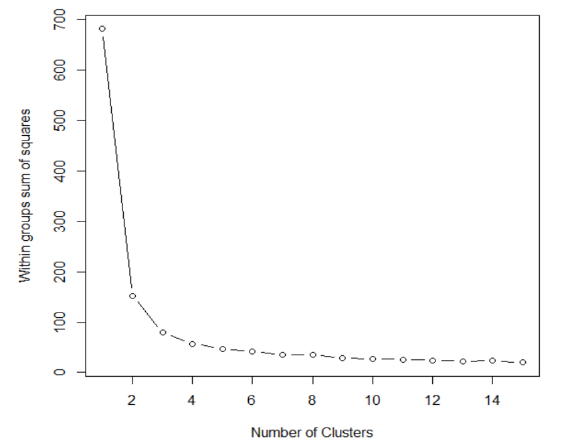
\includegraphics[scale=0.4]{images/chapitre6/elbow_methods.png}
	\end{center}
	\caption{La méthode Elbow.}
	\label{elbow_methods}
\end{figure}

\begin{itemize}
	\item	\textbf{nstart :} avec le nombre donner au paramètre nstart l’algorithme tente plusieurs configuration initial de la position des centroïdes et retient la meilleurs configuration qui minimise la variance des cluster. La valeur par défaut est 1 mais la valeur recommander est 25 par contre cette valeur conduit `a un gaspillage de ressource avec un grand data set.
	\item	\textbf{Iter.max :} le nombre de fois que l’algorithme doit s’exécuter. La valeur par défaut est 10 ce qui permet au centroïdes de converger ver position d’équilibre.
	\item	\textbf{algorithm :} l’algorithme choisit est celui qui donne une plus forte cohérence des clusters. Avec python l’algorithme kmeans++ donne des meilleurs résultats.

\end{itemize}

\section{Fuzzy clustering}
\subsection{Introduction}
Les méthodes de clustering traditionnelles (Hard) se limitent du fait que chaque point de l'ensemble de données appartient à un seul cluster. La théorie des ensembles flous proposée par Zadeh \cite{zadeh1965information} en 1965 a fait jaillir le concept d'incertitude d'appartenance, qui est décrit par la fonction d'appartenance \cite{yang1993survey}. L'utilisation d'ensembles flous fournit des informations d'appartenance de classe imprécises. L'application de la théorie des ensembles flous dans l'analyse de cluster a été proposée pour la première fois dans les travaux de Bellman, Kalaba et Zadeh \cite{zadeh1965information} et Ruspini \cite{ruspini1969new}. \\
Ruspini a proposé l'utilisation d'ensembles flous dans le clustering sous la forme d'une fonction objective qui obtient une meilleure partition floue des données en utilisant des méthodes Fuzzy (flou). Et cette méthode devient un problème d’optimisation de de fonction objective qui appartient à la catégorie du clustering flou basé sur les fonctions objectives. Il existe aussi le clustering flou basé sur une relation floue et le clustering « fuzzy generalized k-nearest neighbor rule ».\\
De nombreuses méthodes de regroupement flou ont été proposées en raison de modifications des fonctions objectives, qui visent à améliorer le résultat en ce qui concerne le bruit, les valeurs aberrantes, etc \cite{zhou2016method}. La méthode la plus utilisée est c-means (FCM) qui est une technique non supervisée qui classe les points de données similaires en clusters \cite{gurrutxaga2010sep}.\\
Dans de nombreuses situations, le clustering Soft est plus naturel que le clustering Hard parce que les objets situés aux limites entre plusieurs classes ne sont pas forcés d'appartenir entièrement à l'un des clusters, mais se voient plutôt attribuer des degrés d'appartenance compris entre 0 et 1 indiquant leur appartenance partielle. Au contraire, dans les techniques de clustering hard, les données sont groupées de manière exclusive, de sorte que si une certaine donnée appartient à un cluster défini, elle ne peut pas être incluse dans un autre cluster \cite{bora2014comparative}. Nous verrons dans cette section le Fuzzy c-means qui est une technique de clustering flou très populaire.\\

\subsection{Fuzzy C-means clustering :}
Fuzzy C-means (FCM) est une technique de regroupement de données dans laquelle chaque point de données appartient à un cluster dans une certaine mesure spécifiée par un degré d'appartenance. Cette technique a été initialement développé par Dunn 1973 et améliorer par Jim Bezdek en 1981 par rapport aux méthodes de clustering antérieures \cite{taherpour2018application}. Il fournit une méthode de regroupement des points de données qui peuplent un espace multidimensionnel dans un nombre spécifique de clusters différents. Le principal avantage de cette methode est qu’elle fournit des appartenances graduelles de points de données à des clusters mesurés en degrés dans un intervalle [0,1]. Cela donne la flexibilité d'exprimer que les points de données peuvent appartenir à plus d'un cluster.
\subsubsection{Algorithme FCM :}
Le but est de minimiser la fonction objective définie comme suit :

\begin{equation}
    J_{m} = \sum_{i=1}^{N} \sum_{j=1}^{C} U_{ij}^{m} \left\lVert x_{i} - c_{j} \right\rVert^{2} \hspace{10pt} avec \hspace{10pt}  1 \leq m \textless \infty
\end{equation}
Où \(\displaystyle U_{ij} \) est le degré auquel une observation \(\displaystyle x_{i} \) appartient à un cluster \(\displaystyle j \), \(\displaystyle c_{j} \) est le centre du cluster \(\displaystyle j \) et \(\displaystyle m \) le fuzzifier.

On remarque que FCM differe de k-means  du fait que FCM utilise les valeurs d’appartance \(\displaystyle U_{ij} \) et le fuzzifier \(\displaystyle m \). La variable \(\displaystyle U_{ij}^{m} \) est inversement lié à la distance entre x et le centre de cluster et est défini par  :
\begin{equation}
    U_{ij}^{m} = \frac{1}{\sum_{k=1}^{C} \Bigg ( \frac{\left\lVert x_{i} - c_{j} \right\rVert }{\left\lVert x_{i} - c_{k} \right\rVert} \Bigg )^{\frac{2}{m-1}}}
\end{equation}
Le paramètre \(\displaystyle m \) est un nombre réel supérieur à 1 \(\displaystyle (1 \leq m \textless \infty) \) et il définit le niveau de flou du cluster. Une valeur de \(\displaystyle m \) proche de 1 donne une solution de cluster qui devient de plus en plus similaire à la solution de clustering \textbf{Hard} tel que k-means ; alors qu’une valeur de m proche de l’infini conduit à un flou complet. Le bon choix est d’utiliser \(\displaystyle m = 2.0 \) \cite{hathaway2001fuzzy}. \\
Enfin le centroïde d’un cluster est la moyenne de tous les points, pondérée par leur degré d’appartenance au cluster. 

\begin{equation}
    C_{j} = \frac{\sum_{i = 1}^{N} U_{ij}^{m} \cdot x_{i}}{ \sum_{i=1}^{N} U_{ij}^{m}}
\end{equation}

\begin{figure}[!h]
    \centering
    \subfloat[\centering Les éléments du dataset Iris \cite{iris_dataset}.]{{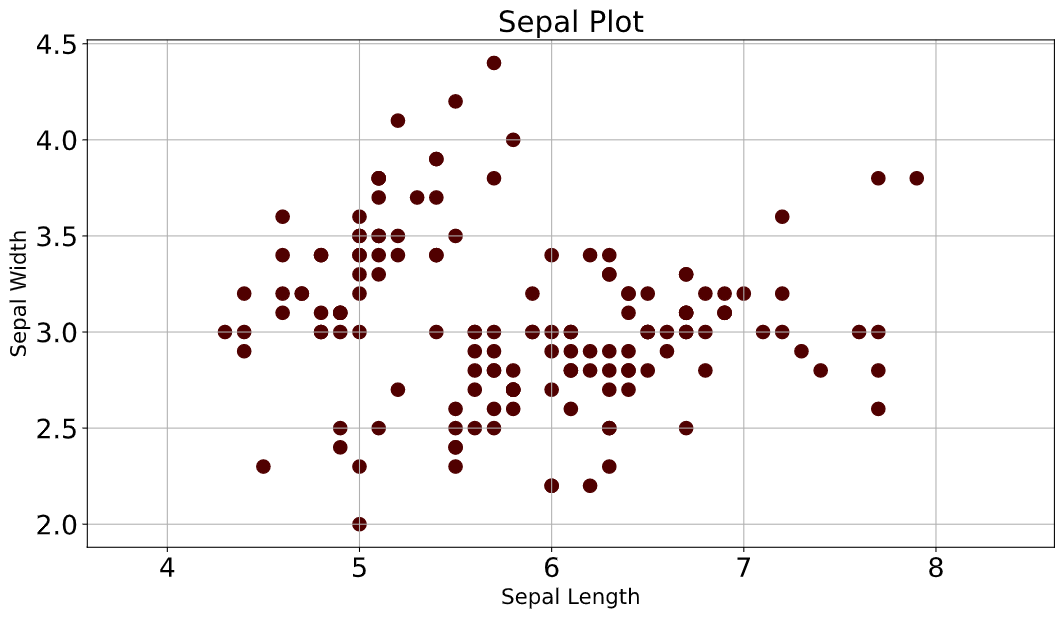
\includegraphics[width=7cm]{images/chapitre6/data_for_fuzzy.png} \label{data_for_fuzzy} }}%
    \qquad
    \subfloat[\centering Illustration du degré d’appartenance des éléments au cluster.]{{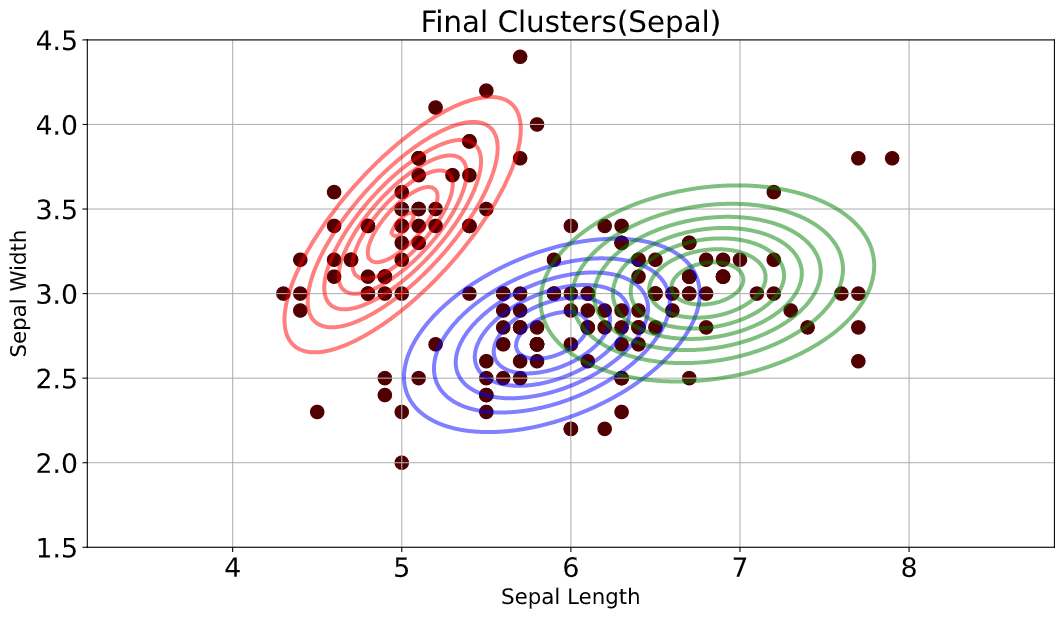
\includegraphics[width=7cm]{images/chapitre6/fuzzyExemple.png} } \label{fuzzy_example}}%
    %\caption{Dendrogramme}%
\end{figure}

\subsection{Conclusion}
Le clustering flou c-means peut être considéré comme un meilleur algorithme par rapport à l'algorithme k-Means. Contrairement à l'algorithme k-Means où les points de données appartiennent exclusivement à un cluster, dans le cas de l'algorithme flou c-means, le point de données peut appartenir à plus d'un cluster avec une vraisemblance ou une probabilité. Le regroupement flou c-means donne des résultats comparativement meilleurs pour les ensembles de données qui se chevauchent.

\section{Les autres méthodes de clustering}
En dehors des méthodes de clustering hiérarchique, partitionnel et floue (fuzzy) vu précédemment, les autres méthodes de clustering sont énoncées de façon brève dans le tableau \ref{other_clustering_methods} . 
\begin{table}[H]
	\centering
	\addtolength{\leftskip} {-3cm}
	\addtolength{\rightskip}{-4cm}
	\begin{tabular}{|m{3cm}|m{4cm}|m{4cm}|m{3cm}|m{2cm}|} %\rule{0pt}{1.5\normalbaselineskip}
	\hline
	\rowcolor{blueforest}
	\color{white} \textbf{Clustering Method} & \color{white} \textbf{Description} & \color{white} \textbf{Advantages} & \color{white} \textbf{Disadvantages} & \color{white} \textbf{Algorithms}\\
	\hline\hline
	\textbf{Distribution based Clustering}  & Basé sur la distribution de probabilité des données, les clusters sont dérivés de diverses métriques telles que la moyenne, la variance, etc. & Le nombre de clusters n'a pas besoin d'être spécifié a priori, fonctionne sur des données en temps réel, les métriques sont faciles à comprendre et à régler. & Algorithme complexe et lent, ne peut pas être adapté à des données plus volumineuses & Gaussian Mixed Models, DBCLASD\\ \hline
	\textbf{Density based Clustering (Model-based methods)} & Basé sur la densité des points de données, également connu sous le nom de clustering basé sur un modèle. & Peut gérer le bruit et les valeurs aberrantes, n'a pas besoin de spécifier le nombre de clusters au début, les clusters créés sont très homogènes, aucune restriction sur les formes de cluster.  & Algorithme complexe et lent, ne peut pas être adapté à des données plus volumineuses & DENCAST, DBSCAN \\ \hline
	\textbf{Constraint based (Supervised Clustering)} & Le clustering est dirigé et contrôlé par les contraintes & Crée une limite de décision parfaite, peut déterminer automatiquement les classes de résultats en fonction des contraintes, les données futures peuvent être classées en fonction des limites de formation. & Surapprentissage, niveau élevé d'erreurs de classification erronée, ne peut pas être entraîné sur des ensembles de données plus volumineux & Decision Trees, Random Forest, Gradient Boosting. \\ \hline
	\end{tabular}
	\caption{Les autres méthodes de clustering}
	\label{other_clustering_methods}
\end{table}

\section{La différence entre le clustering hiérarchique, partitionnel et Fuzzy clustering}
Le clustering hiérarchique et partitionnel présentent des différences essentielles en termes de temps d’exécution, d’hypothèses, de paramètres d’entrée et de clusters résultants. En règle générale, le clustering partitionnel est plus rapide que le clustering hiérarchique. La classification hiérarchique nécessite uniquement une mesure de similarité, tandis que la classification partitionnelle requiert des hypothèses plus strictes telles que le nombre de classes et les centres initiaux. La mise en cluster hiérarchique ne nécessite aucun paramètre d’entrée, tandis que les algorithmes de mise en cluster partiels nécessitent le nombre de clusters à exécuter. La classification hiérarchique renvoie une division beaucoup plus significative et subjective des grappes, mais la classification partitionnelle produit exactement k clusters. Les algorithmes de classification hiérarchique conviennent mieux aux données catégoriques, à condition qu’une mesure de similarité puisse être définie en conséquence. En terme générale ils sont considérés comme des méthodes de clustering Hard, où chaque élément est affecté à un seul cluster. Par contre les méthodes de clustering Soft comme le Fuzzy clustering regroupent les éléments de données de telle sorte qu'un élément puisse exister dans plusieurs clusters.
\section{Indice de validité du clustering}
Les algorithmes supervisés ont beaucoup de métriques pour vérifier leur qualité d'ajustement comme la précision, la valeur \(\displaystyle R^{2}\), la sensibilité, la spécificité, etc. Concernant les algorithmes non supervisés et plus précisément les algorithmes de clustering l’indice de validité de cluster est utilisé pour mesurer la qualité de la partition trouvée et aussi les partitions optimales. L’indice de validité de cluster est utilisé donc pour mesurer la qualité des clusters et pour rechercher le nombre optimal de clusters lorsque le nombre de clusters dans les données l'ensemble n'est pas connu à l'avance \cite{rezaee1998new}. Il utilise les propriétés des clusters telles que la compacité (ou la variation) et la séparation (ou l'isolement) qui sont souvent considérées comme des caractéristiques majeures permettant de valider les clusters. La compacité indique la variation ou la dispersion des données au sein d'un cluster, et la séparation indique l'isolement des clusters les uns des autres \cite{ZHANG20081205} . Plusieurs indices de validité courants sont énoncés dans le tableau suivant :
\begin{table}[H]
	\centering
	\addtolength{\leftskip} {-4cm}
	\addtolength{\rightskip}{-4.5cm}
	\begin{tabular}{|m{2cm}|m{5cm}|m{10cm}|}
	\hline
	\rowcolor{blueforest}
	\color{white} \textbf{Indice} & \color{white} \textbf{Description} & \color{white} \textbf{Formule}  \\
	\hline\hline
	\multicolumn{3}{|m{17cm}|}{\centering \textbf{Les indices de validité adaptés aux clustering partitionnelle} }\\ \hline
	\textbf{Indice de Dunn}  &
	Il est l'un des indices les plus anciens et les plus cités est proposé par \cite{dunn1974well}. L'index de Dunn (DU) identifie les clusters qui sont bien séparés et compacts. Le but est donc de maximiser la distance inter-clusters tout en minimisant la distance intra-cluster. &  \(\displaystyle DU_{k} = \min_{i=1,..,k} \Bigg \{ \min_{j=1+1,..,k} \Bigg ( \frac{diss(c_{i},c_{j})}{\max_{m=1,...,k}diam(c_{m})} \Bigg ) \Bigg \} \) \newline \newline où \(\displaystyle diss(c_{i},c_{j}) = \min_{x \in c_{i},y \in c_{j}}d(x,y) \) est la dissemblance entre les clusters \(\displaystyle c_{i} \) et \(\displaystyle c_{j}  \), et \(\displaystyle diam(C) = \max_{x,y \in C}d(x,y) \) est la fonction intra-cluster (ou diamètre) du cluster. Si l'index de Dunn est grand, cela signifie qu'il existe des clusters compacts et bien séparés \cite{Saitta2008}. \\ \hline
	\textbf{Indice Calinski-Harabasz}  &
	Cet indice \cite{calinski1974dendrite} est basé sur un rapport entre la matrice de dispersion des clusters (BCSM) et la matrice de dispersion des clusters (WCSM). &  \(\displaystyle CH_{k} = \frac{BCSM}{k-1} \cdot \frac{n-k}{WCSM} \) \newline où \(\displaystyle n  \) est le nombre total de points et \(\displaystyle k  \) le nombre de clusters. Le \(\displaystyle BCSM   \) est basé sur la distance entre les clusters et est défini par : \(\displaystyle BCSM = \sum_{i=1}^{k} n_{i} \cdot d(z_{i},z_{tot})^{2}  \), où \(\displaystyle z_{i}  \) est le centre du cluster \(\displaystyle c_{i}  \) et \(\displaystyle n_{i}  \) le nombre de points dans \(\displaystyle c_{i}  \). Le \(\displaystyle WCSM  \)  est : \(\displaystyle WCSM = \sum_{i=1}^{k} \sum_{x \in c_{i}} d(x,z_{i})^{2}  \) où \(\displaystyle x  \) x est un point de données appartenant au cluster \(\displaystyle c_{i}  \). Pour obtenir des clusters bien séparés et compacts, BCSM est maximisé et WCSM minimisé \cite{Saitta2008}. \\ \hline
	\textbf{Indice Davies-Bouldin} & Semblable à l'indice de Dunn, l'indice Davies-Bouldin \cite{davies1979cluster} identifie des clusters éloignés les uns des autres et compacte.  & \(\displaystyle DB_{k} = \frac{1}{k} \sum_{i=1}^{k} max_{j=1,...,k;i \neq j} \Bigg \{ \frac{diam(c_{i}) + diam(c_{j})}{d(z_{i},z_{j})} \Bigg \}  \) \newline où le diamètre d'un cluster est : \(\displaystyle diam(c_{i}) = \sqrt{\frac{1}{n_{i}} \sum_{x \in c_{i}} d(x,z_{i})^{2}}  \), avec \(\displaystyle n_{i}  \) le nombre de points et \(\displaystyle z_{i}  \) le centre de gravité du cluster \(\displaystyle c_{i}  \). Puisque l'objectif est d'obtenir des clusters avec des distances intra-clusters minimales, les petites valeurs de \(\displaystyle DB  \) sont intéressantes. Par conséquent, cet index est minimisé lors de la recherche du meilleur nombre de clusters \cite{Saitta2008}. \\ \hline
	\textbf{Indice de silhouette} & La statistique de silhouette \cite{kaufman2009finding} est une autre façon bien connue d'estimer le nombre de groupes dans une donnée ensemble. L'indice Silhouette (SI) calcule pour chaque point une largeur en fonction de son appartenance à groupe. Cette largeur de silhouette est alors une moyenne sur l'ensemble des observations.  & \(\displaystyle SI_{k} = \frac{1}{k} \sum_{i=1}^{n} \frac{(b_{i} - a_{i})}{\max (a_{i},b_{i})}  \), \newline où \(\displaystyle n  \) est le nombre total de points, \(\displaystyle a_{i}  \) est la distance moyenne entre le point \(\displaystyle i  \) et tous les autres points de son propre cluster et \(\displaystyle b_{i}  \) est le minimum des dissemblances moyennes entre \(\displaystyle i  \) et les points d'autres clusters. Enfin, la partition avec le \(\displaystyle SI  \) le plus élevé est considérée comme optimale \cite{Saitta2008}. \\ \hline
	\end{tabular}
	\caption{Indice de validité du clustering Hard}
	\label{validity_index_hard}
\end{table}

\begin{table}[H]
	\centering
	\addtolength{\leftskip} {-4cm}
	\addtolength{\rightskip}{-4.5cm}
	\begin{tabular}{|m{7cm}|m{10cm}|}
	\hline
	\rowcolor{blueforest}
	\color{white} \textbf{Indice} & \color{white} \textbf{Formule}  \\
	\hline\hline
	\multicolumn{2}{|m{17cm}|}{Il y’a aussi d’autre indice de validité de clustering partitionnel comme l’indice de Maulik-Bandyopadhyay et Geometric index. Les indices de validité utilisé pour le fuzzy clustering sont : }\\ \hline
	  \textbf{Le coefficient de partition \(\displaystyle PC \) \cite{bezdek1974numerical} }  & \(\displaystyle V_{PC} = \frac{1}{n} \sum_{i=1}^{c} \sum_{j=1}^{n} u_{ij}^{2} \) \\ \hline
	  \textbf{L'entropie de partition \(\displaystyle PE \) \cite{bezdek1973cluster} }  & \(\displaystyle V_{PE} = - \frac{1}{n} \sum_{i=1}^{c} \sum_{j=1}^{n} u_{ij} \log u_{ij} \) \\ \hline
	  \textbf{Fonction de validité proposée par Wu et Yang \cite{wu2005cluster} }  & \(\displaystyle V_{PCAES} = \sum_{i=1}^{c} PCAES_{i} = \sum_{i=1}^{c} \sum_{j=1}^{n}u_{ij}^{2}/u_{M} - \sum_{i=1}^{c} \exp (- \min_{k \neq i} \{ \left\lVert v_{i} - v_{k} \right\rVert^{2} / \beta_{T}   \} ) \) \newline où \(\displaystyle u_{M} = \min_{1 \leq i \leq  c} \Bigg \{ \sum_{j=1}^{n} u_{ij}^{2} \Bigg \}\), \(\displaystyle \beta_{T} = \frac{\sum_{l=1}^{c} \left\lVert v_{l} - \overline{v} \right\rVert^{2} }{c}   \) et \(\displaystyle \overline{v} = \sum_{j=1}^{n} x_{j}/n  \) \newline La grande valeur VPCAES signifie que les \(\displaystyle c  \) clusters sont compact et séparé les uns des autres, et la petite valeur VPCAES implique qu’ils ne sont pas compacts ou séparés.  \\ \hline
	  \textbf{Fonction de validité proposée par Fukuyama et Sugeno \cite{fukuyama1989new} }  & \(\displaystyle V_{FS} = J_{m}(U,V) - K_{m}(U,V) = \sum_{i=1}^{c}\sum_{j=1}^{n} u_{ij}^{m} \left\lVert x_{j} - v_{i} \right\rVert^{2} - \sum_{i=1}^{c}\sum_{j=1}^{n} u_{ij}^{m} \left\lVert v_{i} - \overline{v} \right\rVert^{2} \) , \newline où \(\displaystyle \overline{v} = \sum_{j=1}^{n} x_{j}/n \) . \\ \hline
	  \textbf{Fonction de validité proposée par Xie et Beni \cite{xie1991validity}  }  & \(\displaystyle V_{XB} = \frac{J_{m}(U,V)/n}{Sep(V)} = \frac{\sum_{i=1}^{c}\sum_{j=1}^{n} u_{ij}^{m} \left\lVert x_{j} - v_{i} \right\rVert^{2} }{n\min_{i \neq j} \left\lVert v_{i} - v_{j} \right\rVert^{2} } \) \\ \hline
	\end{tabular}
	\caption{Indice de validité du clustering Soft}
	\label{validity_index_soft}
\end{table}


\section{Conclusion}
Nous avons passé en revue dans cette partie le clustering qui est une méthode de l’apprentissage automatique non-supervisé et les techniques qu’il utilise pour l’extraction des clusters. Plusieurs objectif pousse à utiliser certaines techniques de clustering comme le clustering partitionnel et hiérarchique qui forme des clusters où chaque élément appartient à un seul cluster et le clustering flou (fuzzy) où chaque élément peut appartenir à plusieurs clusters avec un degré d’appartenance. Ensuite après l’extraction des clusters, les indices de validité de clusters peuvent être utilisé pour évaluer la qualité des clusters obtenue où détecter à l’avance le nombre de clusters optimale avant d’utiliser les algorithmes.